\documentclass[journal,10pt]{IEEEtran}
\usepackage{amsmath,amssymb}
\usepackage{newtxtext,newtxmath}
\usepackage{booktabs,graphicx,longtable,microtype,url}
\usepackage[hidelinks]{hyperref}
\setlength{\emergencystretch}{2em}
\newcommand{\ControlledN}{397}
\newcommand{\ControlledChunks}{34,193}
\newcommand{\ControlledSources}{2,956}
\newcommand{\ControlledPriorAP}{0.6090}
\newcommand{\ControlledQCRAP}{0.8425}
\newcommand{\ControlledAPDelta}{0.2335}
\newcommand{\ControlledAPLower}{0.1850}
\newcommand{\ControlledAPUpper}{0.2841}
\newcommand{\ControlledPriorHit}{0.7683}
\newcommand{\ControlledQCRHit}{0.9446}
\newcommand{\ExternalN}{219}
\newcommand{\ExternalPriorAP}{0.5408}
\newcommand{\ExternalQCRAP}{0.7020}
\newcommand{\ExternalAPDelta}{0.1612}
\newcommand{\ExternalAPLower}{0.0911}
\newcommand{\ExternalAPUpper}{0.2334}
\newcommand{\ExternalPriorHit}{0.6256}
\newcommand{\ExternalQCRHit}{0.7534}
\newcommand{\ExternalIndex}{72.77}
\newcommand{\NaturalVideos}{5,359}
\newcommand{\NaturalEvents}{35,625}
\newcommand{\NaturalCLAPMAP}{0.067576}
\newcommand{\NaturalQCRMAP}{0.052603}
\newcommand{\NaturalCLAPFourMAP}{0.052280}
\newcommand{\NaturalDeltaPoints}{-1.4973}
\newcommand{\NaturalVideoDeltaPoints}{-1.1334}
\newcommand{\NaturalVideoLowerPoints}{-1.4749}
\newcommand{\NaturalVideoUpperPoints}{-0.7804}
\newcommand{\NaturalWorstClassPoints}{-7.1301}
\newcommand{\RouterMAP}{0.096995}
\newcommand{\RouterDeltaPoints}{2.9419}
\newcommand{\RouterRelativeGain}{43.53}
\newcommand{\RouterVideoDeltaPoints}{6.2251}
\newcommand{\RouterVideoLowerPoints}{5.8165}
\newcommand{\RouterVideoUpperPoints}{6.6397}
\newcommand{\CLAPRouterMAP}{0.093921}
\newcommand{\CLAPRouterDeltaPoints}{2.6345}
\newcommand{\IncrementalMAPPoints}{0.3074}
\newcommand{\IncrementalGainShare}{10.45}
\newcommand{\IncrementalVideoPoints}{1.3737}
\newcommand{\IncrementalVideoLowerPoints}{1.1571}
\newcommand{\IncrementalVideoUpperPoints}{1.5895}
\newcommand{\QCRAssignmentPercent}{30.0}
\newcommand{\ActionFormerMAP}{0.116638}
\newcommand{\ActionFormerGapPoints}{1.9643}
\newcommand{\FullPreCapRows}{1,453,945}
\newcommand{\FullFinalRows}{1,044,156}
\newcommand{\FullDiscardedRows}{409,789}
\newcommand{\FullVideosOverCap}{4,401}
\newcommand{\FullMaxPreCap}{356}
\newcommand{\CLAPPreCapRows}{1,662,296}
\newcommand{\CLAPFinalRows}{1,069,264}
\newcommand{\CLAPDiscardedRows}{593,032}
\newcommand{\CLAPVideosOverCap}{5,119}
\newcommand{\CLAPMaxPreCap}{389}
\newcommand{\AnswerSelected}{0.4586}
\newcommand{\AnswerCLAP}{0.4619}
\newcommand{\AnswerStrongest}{0.4780}
\newcommand{\AnswerRandom}{0.4731}
\newcommand{\AnswerOracle}{0.4886}
\newcommand{\AnswerSilence}{0.3877}
\newcommand{\AnswerTextOnly}{0.4033}
\newcommand{\AnswerVsStrongestPoints}{-1.9444}
\newcommand{\AnswerVsStrongestLowerPoints}{-5.2778}
\newcommand{\AnswerVsStrongestUpperPoints}{1.4111}
\newcommand{\UpstreamMaximumDifference}{0.00001873}
\newcommand{\UpstreamReproductionDifference}{5.55e-17}


\title{Supplement: Where Query-Conditioned Audio Ranking Transfers---and Where It Fails}
\author{Author metadata required before submission}

\begin{document}
\maketitle

\begin{table*}[t]
\caption{Frozen and diagnostic conjunctions.}
\centering
\scriptsize
\begin{tabular}{p{0.21\textwidth}p{0.57\textwidth}r}
\toprule
Stage & Gate & Result\\
\midrule
Controlled exact-onset &
AP gain $\ge0.05$; Hit@1 gain $\ge0.05$; both bootstrap lower bounds
$>0$; at least four positive seeds; no condition Hit@1 loss below $-0.05$;
integrity & 7/7 pass\\
External exact-onset &
Controlled gates plus no class Hit@1 loss below $-0.05$ and performance index
$\ge85$ & 7/8; index \ExternalIndex\\
Frozen natural transfer &
global delta $>0$; video lower bound $>0$; at least four positive thresholds;
worst class $\ge-0.05$; QCR multi $\ge$ CLAP 4 s; integrity & 2/6 fail\\
Cap-correct diagnosis &
global delta $>0$; video lower bound $>0$; threshold breadth; class non-harm;
10 exact cap reconstructions; 50 assignments; integrity & 7/7 met\\
Answer bridge &
gain over strongest and random; backbone non-harm; response/content and
integrity checks & 5/8 fail\\
\bottomrule
\end{tabular}
\end{table*}

\section{Controlled and external exact-onset results}
\begin{table*}[t]
\caption{Evidence-ranking metrics. Bootstrap intervals are paired at the
recipe or original-source unit declared by each protocol.}
\centering
\footnotesize
\begin{tabular}{lrrrrrr}
\toprule
Panel & Recipes & Prior AP & QCR AP & AP difference (95\% interval) &
Prior Hit@1 & QCR Hit@1\\
\midrule
Source-isolated confirmation & \ControlledN & \ControlledPriorAP &
\ControlledQCRAP & \ControlledAPDelta\
[\ControlledAPLower,\ControlledAPUpper] &
\ControlledPriorHit & \ControlledQCRHit\\
External source-disjoint & \ExternalN & \ExternalPriorAP & \ExternalQCRAP &
\ExternalAPDelta\ [\ExternalAPLower,\ExternalAPUpper] &
\ExternalPriorHit & \ExternalQCRHit\\
\bottomrule
\end{tabular}
\end{table*}

The source-isolated panel contains \ControlledChunks\ chunks from
\ControlledSources\ unique source files and has zero development source
overlap. The external panel excludes every UrbanSound8K Freesound ID found in
ESC-50 metadata and uses LibriSpeech \texttt{test-other} backgrounds. Its
relative AP and Hit@1 intervals exclude zero, but the prespecified absolute
performance index is \ExternalIndex\ rather than 85.

\section{Frozen natural outcome}
\begin{table}[t]
\caption{Natural zero-shot gate observations.}
\centering
\footnotesize
\begin{tabular}{lrl}
\toprule
Gate & Observed & Decision\\
\midrule
Global mAP difference $>0$ & \NaturalDeltaPoints\ pp & Fail\\
Video-bootstrap lower $>0$ & \NaturalVideoLowerPoints\ pp & Fail\\
Positive thresholds $\ge4$ & 0/5 & Fail\\
Worst class $\ge-5$ pp & \NaturalWorstClassPoints\ pp & Fail\\
QCR multi $\ge$ CLAP 4 s & \NaturalQCRMAP\ vs.\ \NaturalCLAPFourMAP & Pass\\
Integrity & zero failures & Pass\\
\bottomrule
\end{tabular}
\end{table}

The complete-prediction sensitivity to pinned upstream ActionFormer sorting
and tIoU arithmetic has maximum mAP difference
\UpstreamMaximumDifference. Reproducing both upstream semantics locally
matches within \UpstreamReproductionDifference\ and leaves every
metric-dependent gate unchanged.

\section{Cap-corrected cross-fitting details}
Each candidate pool retains at most 50 segments per class before shared video
capping. Reapplying the frozen sort and 200-segment video cap reconstructs all
ten original candidate files exactly. For held fold $f$ and class $c$, the
candidate is selected on all folds except $f$; class streams are joined only
after selection and capped once.

\begin{table*}[t]
\caption{Fold-by-class selections. C denotes CLAP, Q denotes QCR, and MS denotes pooled multiscale.}
\centering
\scriptsize
\begin{tabular}{llccccc}
\toprule
Class & Candidate family & Fold 0 & Fold 1 & Fold 2 & Fold 3 & Fold 4\\
\midrule
Human:Speech & CLAP+QCR & Q-4 & Q-4 & Q-4 & Q-4 & Q-4\\
Human:Speech & CLAP-only & C-MS & C-MS & C-MS & C-MS & C-MS\\
Animal:sound & CLAP+QCR & Q-4 & Q-4 & Q-4 & Q-4 & Q-4\\
Animal:sound & CLAP-only & C-4 & C-4 & C-4 & C-4 & C-4\\
Object:opening/closing of something & CLAP+QCR & C-2 & C-2 & C-2 & C-2 & C-2\\
Object:opening/closing of something & CLAP-only & C-2 & C-2 & C-2 & C-2 & C-2\\
Object:sound & CLAP+QCR & C-2 & C-2 & C-2 & C-2 & C-2\\
Object:sound & CLAP-only & C-2 & C-2 & C-2 & C-2 & C-2\\
Human:Sound(clapping) & CLAP+QCR & C-0.5 & C-0.5 & C-0.5 & C-0.5 & C-0.5\\
Human:Sound(clapping) & CLAP-only & C-0.5 & C-0.5 & C-0.5 & C-0.5 & C-0.5\\
Interaction: fluid & CLAP+QCR & C-2 & C-2 & C-2 & C-2 & C-2\\
Interaction: fluid & CLAP-only & C-2 & C-2 & C-2 & C-2 & C-2\\
Interaction:dropping & CLAP+QCR & Q-1 & Q-1 & Q-1 & Q-1 & Q-1\\
Interaction:dropping & CLAP-only & C-1 & C-1 & C-1 & C-1 & C-1\\
Interaction:hitting & CLAP+QCR & C-1 & C-1 & C-1 & C-1 & C-1\\
Interaction:hitting & CLAP-only & C-1 & C-1 & C-1 & C-1 & C-1\\
Interaction:rolling & CLAP+QCR & C-1 & C-1 & C-1 & C-1 & C-2\\
Interaction:rolling & CLAP-only & C-1 & C-1 & C-1 & C-1 & C-2\\
Object:breaking of something & CLAP+QCR & C-4 & C-4 & C-4 & C-4 & C-4\\
Object:breaking of something & CLAP-only & C-4 & C-4 & C-4 & C-4 & C-4\\
\bottomrule
\end{tabular}
\end{table*}


\begin{table*}[t]
\caption{Output-cap audit.}
\centering
\footnotesize
\begin{tabular}{lrrrrr}
\toprule
Route & Pre-cap rows & Final rows & Discarded & Videos over 200 & Max pre-cap\\
\midrule
CLAP+QCR & \FullPreCapRows & \FullFinalRows & \FullDiscardedRows &
\FullVideosOverCap & \FullMaxPreCap\\
CLAP-only & \CLAPPreCapRows & \CLAPFinalRows & \CLAPDiscardedRows &
\CLAPVideosOverCap & \CLAPMaxPreCap\\
\bottomrule
\end{tabular}
\end{table*}

The full-versus-fixed-CLAP paired video interval is
[\RouterVideoLowerPoints,\RouterVideoUpperPoints] percentage points. The
post-hoc incremental full-versus-CLAP-only interval is
[\IncrementalVideoLowerPoints,\IncrementalVideoUpperPoints] points. These
video-macro effects are not algebraically identical to global class-macro
mAP differences.

\section{All natural class effects}
\begin{table*}[t]
\caption{Class mean AP and cross-fit decomposition.}
\centering
\scriptsize
\begin{tabular}{lrrrrr}
\toprule
Class & Fixed CLAP & CLAP-only & Full & Full$-$fixed & Full$-$CLAP-only\\
\midrule
Human:Speech & 0.082197 & 0.082996 & 0.101187 & 0.018990 & 0.018191\\
Animal:sound & 0.005356 & 0.021934 & 0.026341 & 0.020985 & 0.004407\\
Object:opening/closing of something & 0.010656 & 0.015561 & 0.016328 & 0.005673 & 0.000767\\
Object:sound & 0.041209 & 0.057493 & 0.059273 & 0.018064 & 0.001780\\
Human:Sound(clapping) & 0.199148 & 0.279395 & 0.279408 & 0.080260 & 0.000014\\
Interaction: fluid & 0.134348 & 0.248483 & 0.248969 & 0.114621 & 0.000487\\
Interaction:dropping & 0.022112 & 0.034267 & 0.034968 & 0.012855 & 0.000701\\
Interaction:hitting & 0.132861 & 0.147388 & 0.151216 & 0.018355 & 0.003828\\
Interaction:rolling & 0.045023 & 0.045280 & 0.045487 & 0.000464 & 0.000207\\
Object:breaking of something & 0.002854 & 0.006413 & 0.006772 & 0.003918 & 0.000359\\
\bottomrule
\end{tabular}
\end{table*}


Every full-router class mean AP is above fixed multiscale CLAP. Every
full-router class is also above the CLAP-only router, although several
increments are very small. This is descriptive post-outcome evidence, not ten
independent confirmatory tests.

\section{Downstream answer boundary}
\begin{figure}[t]
\centering
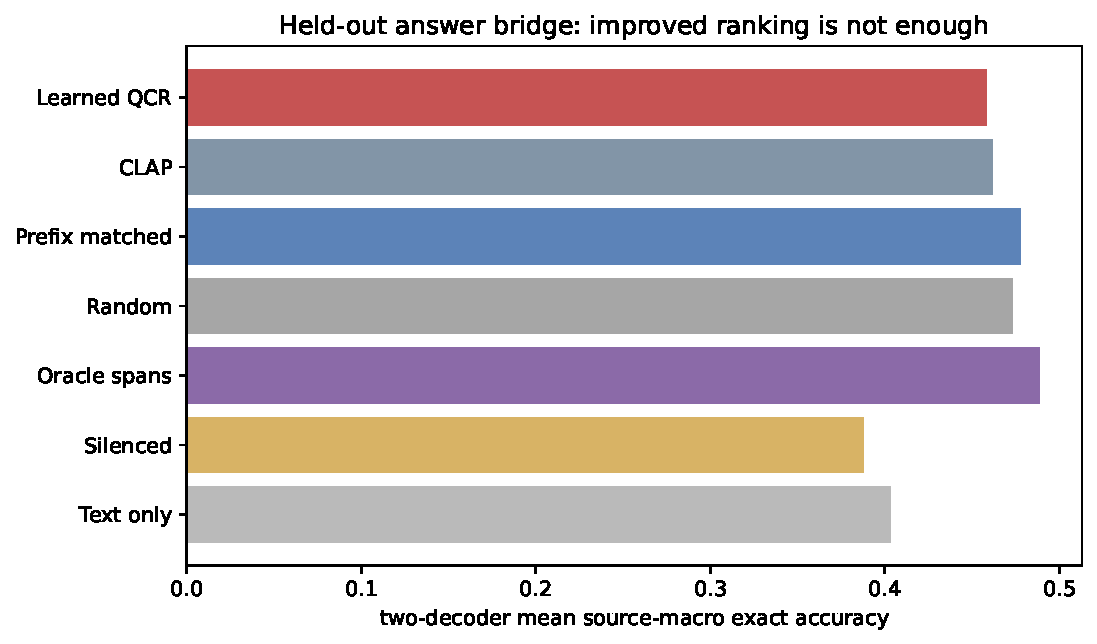
\includegraphics[width=\columnwidth]{extended_figures/AEF05.pdf}
\caption{Two-decoder mean source-macro exact answer accuracy. Oracle spans are
context, not an eligible learned comparator.}
\end{figure}

\begin{table}[t]
\caption{Held-out answer results.}
\centering
\footnotesize
\begin{tabular}{lr}
\toprule
Retriever & Exact accuracy\\
\midrule
Learned QCR & \AnswerSelected\\
CLAP & \AnswerCLAP\\
Prefix matched & \AnswerStrongest\\
Deterministic random & \AnswerRandom\\
Oracle spans & \AnswerOracle\\
Silenced selected spans & \AnswerSilence\\
Text only & \AnswerTextOnly\\
\bottomrule
\end{tabular}
\end{table}

The learned-minus-prefix difference is \AnswerVsStrongestPoints\ percentage
points with 95\% source-bootstrap interval
[\AnswerVsStrongestLowerPoints,\AnswerVsStrongestUpperPoints]. AUDITA remains
sealed and is not used to repair the failed bridge.

\section{Invalidations and amendments}
\begin{itemize}
  \item The first cross-fit proposal joined per-class outputs that had each
  already passed a video cap. This could exceed 200 segments after joining.
  The analyzer was stopped before a router report; the observed candidate
  mAP values and defect are retained in
  \texttt{INVALIDATION\_OUTPUT\_CAP.md}.
  \item The corrected track rebuilds uncapped per-class pools, reconstructs
  all ten source caps exactly, routes classes, and applies one shared cap.
  \item Before router scoring, a quadratic per-video cap assertion was
  replaced by an equivalent single-pass counter. The amendment changes no
  candidate, selection, metric, bootstrap, or cap parameter.
  \item Candidate-pool files are large regenerable intermediates and remain
  outside the compact submission ZIP. Their exact row counts and SHA-256
  values are included. Final full and CLAP-only predictions are included.
\end{itemize}

\section{Reproduction map}
\begin{itemize}
  \item \texttt{q1\_plus/}: controlled confirmation and answer-bridge
  reports, frozen checkpoints, and relevant analysis code.
  \item \texttt{q1\_90/}: external exact-onset protocol, recipes, report, and
  acquisition/rights records.
  \item \texttt{q1\_top\_tier/}: natural freeze, prediction reports, metric
  audit, supervised contextual receipt, and source.
  \item \texttt{q1\_crossfit\_capcorrect/}: cap-correct locks, candidate
  receipt, final predictions, report, tests, and publication analysis.
  \item \texttt{figure\_source\_data/}: source rows for every figure.
\end{itemize}

\end{document}
